\chapter{MPI GE CMIP6}
\label{ch:dataset}

The dataset chosen for this project is the \textit{Max Planck Institute Grand Ensemble CMIP6} (from now on MPI-GE CMIP6), presented by \citeauthor{olonscheck_new_2023}. 
It is a Single-model initial-condition large ensemble (in short: SMILE) consisting of multiple coupled models: ECHAM6 for the atmosphere directly coupled to JSBACH for land and MPIOM for sea and sea-ice. 
The models are coupled once a day, meaning that the simulation results serve as inputs for the other models. 
This means that a single model was run with different initial conditions but the same external forcings (e.g. greenhous gasses) mutiple times. 
Every seperate intial condition is a member of the simulation, and all members together are the whole ensemble. \cite{olonscheck_new_2023}

Following this, every variable/field of the dataset can be interpreted as a uncertain field (see Section~\ref{sec:uncertainfields}).
Combining the members into an ensemble makes it possible to seperate the internal variability from the responses to the external forcing, enabling researchers to better quantify the consequences of climate change (for example). 
Additionally it makes the research of extreme weather phenomena (e.g. droughts, floods etc.) more robust in spite of their rare occurences \cite{maher_large_2021}. 
% As described in Section \ref{sec:climate}, Coupled models 


Since MPI GE CMIP6 follows the CMIP6 protocol (see Section~\ref{sec:climate} and \cite{eyring_overview_2016}), it implements the DECK core with (amongst others) a quasi-stationary preindustrial control simulation and the historical simulations.
Futhermore it also uses the forcings defined by CMIP6 (like volcanic eruptions, solar circle etc.) for the historical and future simulations (see Section~\ref{sec:scenariomip}).

The historical simulations are split from 1000 year preindustrial control simulation circa 25 years apart for each member, and the results of them in the year 2015 serve as the initial state for each corresponding member in the future scenarios. 

\begin{enumerate}[itemsep=1pt, topsep=2pt]
  \item It uses the latest (6th) phase of the Coupled Model Intercomparison Project (CMIP6)
  \item Compared to its predecessor (MPI-GE \cite{maher_max_2019}) it provides high frequency output (6 hour intervals vs. monthly means), which enables taking short-lived weather events and structures (e.g. atmospheric rivers) into account which would be lost in the calculation of the mean
\end{enumerate}


\section{ScenarioMIP: Future Scenarios and Shared Socioeconomic Pathways}

\label{sec:scenariomip}

Since the goal of this thesis is to evaluate the future patterns of climate change, simulations of the future are necessary. 
Furtunately, CMIP (Phase 3) introduced a project of future climate scenarios (ScenarioMIP) in the 2000s, which define and simulate developments of different anthropogenic drivers of climate change \cite{oneill_scenario_2016}. 
They play an important role in climate research and are since then the source for many figures and assessments in IPCC reports \cite{touzepeiffer_coupled_2020}. 
The different scenarios can be used to assess \enquote{\dots possible changes in the climate system, impacts on society and ecosystems, and the effectiveness of response options such as adaptation and mitigation under a wide range of future outcomes} \cite{oneill_scenario_2016}.
Basically, the differences between them are the forcings introduced by multiple variables, including change of land use, climate change mitigation policies, energy usage, population, economic growth and emissions \cite{riahi_shared_2017}.   
For CMIP6 they extended the old model of RCPs (Representative Concentration Pathways), which were used for CMIP5, by adding so called Shared Socioeconomic Pathways (SSPs). 
These SSPs add socioeconomic reasons for the assumed changes in land use and emissions. 


SSPs are derived from five broad, abstract narratives, which are then quantified in different ways. 
So for example the narrative for SSP1 is: 

\begin{center}
  \enquote{Sustainability – Taking the Green Road (Low challenges to mitigation and adaptation) The world shifts gradually, but pervasively, toward a more sustainable path, emphasizing more inclusive development that respects perceived environmental boundaries. Management of the global commons slowly improves, educational and health investments accelerate the demographic transition, and the emphasis on economic growth shifts toward a broader emphasis on human well-being. Driven by an increasing commitment to achieving development goals, inequality is reduced both across and within countries. Consumption is oriented toward low material growth and lower resource and energy intensity.} \cite{riahi_shared_2017}
\end{center}

while the narrative for SSP5 is:

\begin{center}
  \enquote{Fossil-fueled Development – Taking the Highway (High challenges to mitigation, low challenges to adaptation) This world places increasing faith in competitive markets, innovation and participatory societies to produce rapid technological progress and development of human capital as the path to sustainable development. Global markets are increasingly integrated. There are also strong investments in health, education, and institutions to enhance human and social capital. At the same time, the push for economic and social development is coupled with the exploitation of abundant fossil fuel resources and the adoption of resource and energy intensive lifestyles around the world. All these factors lead to rapid growth of the global economy, while global population peaks and declines in the 21st century. Local environmental problems like air pollution are successfully managed. There is faith in the ability to effectively manage social and ecological systems, including by geo-engineering if necessary.} \cite{riahi_shared_2017}
\end{center}

These narratives are then quantified in multiple dimensions (resource availability, technical development, lifestyle changes, population, economic activity etc.). 
These quantifications then serve as an input for a range of integrated assessment models (IAMs), which turn them into the actual forcings needed (e.g. land and energy use, emissions) \cite{riahi_shared_2017}. 

In the actual scenarios these pathways are combined with the additional radiative forcing (RCP, the earlier version of scenarios in CMIP5), resulting in a matrix which can be seen in Figure~\ref{fig:ssprcp}. 
RCP describes the level of radiative forcing (in $Wm^{-2}$) reached in the year 2100.
Although there are now 35 possible scenarios, \citeauthor{oneill_scenario_2016} defined two different tiers of scenarios ranked by their importance. 
Figure~\ref{fig:ssprcp} lists Tier 1, which are scenarios mostly compareable to the old RCP scenarios. 
These scenarios are available in the MPI GE CMIP6, amongst some of Tier 2. \cite{oneill_scenario_2016, riahi_shared_2017, bottinger_michael_ssp_nodate}

\begin{figure}[bht]
  \begin{center}
    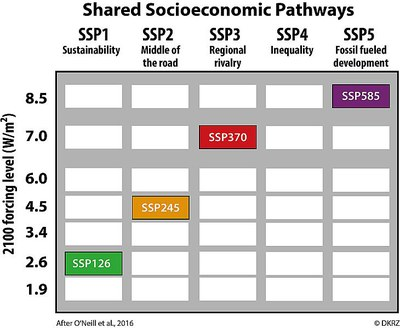
\includegraphics[width=0.5\textwidth]{figures/ssp_rcp_matrix.jpeg}
  \end{center}
  \caption{Combinations of SSPs and RCPs leading to scenarios compareable to the old RCPs \cite{bottinger_michael_ssp_nodate}}
  \label{fig:ssprcp}
\end{figure}


\section{Dataset description}




\subsection{Resolutions and Dimensions}

In terms of spatial resolution, MPI GE CMIP6 comes in three variants: The low resolution variant MPI-ESM1.2-LR with a horizontal resolution of roughly $1.8^\circ$ longitude/latitude resolution in the atmospheric part and $0.4^\circ$ lon/lat for the ocean, the high resolution variant MPI-ESM1.2-HR with a horizontal resolution of $1.0^\circ$/$0.4^\circ$ for atmosphere/ocean and the extreme high resolution MPI-ESM1.2-XR with $0.5^\circ$/$0.4^\circ$ for atmosphere/ocean. 
Each variant has a vertical resolution of 47 levels for the atmosphere and 40 for ocean.
With increasing spatial resolution comes decreased availability of other variables like simulation members, covered time period, and implemented scenarios. 
Although \cite{olonscheck_new_2023} reports 30 members for each simulation (for the LR variant), in the actual dataset available for this work 50 member were simulated. 

In terms of time resolution, MPI GE CMIP6 provides very few, limited variables in 3 hour intervals and most variables in a 6 hour interval.  
A full list of the variables can be seen in \cite[Table 3]{olonscheck_new_2023}, the variables necessary for this thesis are listed in Table~\ref{tab:thesisVariables}. 

\begin{table}[bht]
\centering
\caption{Variables necessary for this thesis, derived from \cite{olonscheck_new_2023}}
\begin{tabular}{l|l|l|l}
  \label{tab:thesisVariables}
\textbf{Name} & \textbf{Parameter Long Name} & \textbf{Unit}                & \multicolumn{1}{l}{\textbf{Vertical Levels}}  \\ 
\hline
\textit{hus}              & Specific Humidity            & $1$                        & 47                                            \\
\textit{ua}               & Eastward (Zonal) Wind        & $ms^{-1}$              & 47                                            \\
\textit{va}               & Westward (Meridional) Wind   & $ms^{-1}$              & 47                                            \\
\textit{ps}               & Surface Air Pressure         & $Pa$                           & 1                                             \\
\textit{pr}               & Precipitation                & $kg~m^{-2} s^{-1}$ & 1                                            
\end{tabular}
\end{table}


\subsection{Vertical Hybrid Sigma Pressure Layers}


Regarding the vertical levels, all variables were not available in fixed pressure layers but in so called \textit{hybrid sigma pressure coordinates}. 
In comparison to fixed pressure layers (like $1000 ~hPa$, $750 ~hPa$\dots), hybrid sigma pressure coordinates follow the terrain (mountains, valleys etc.). 
Essentially, sigma vertical levels are given as fractions of the surface pressure $P_S$ at any point, following the equations in \cite{eckermann_hybrid_2009}: 

\begin{equation}
\label{eq:sigma-definition}
\sigma = h(p,P_S) = \frac{p - P_{top}}{P_S - P_{top}}
\end{equation}

Here $p \in [P_S, P_{top}]$ is a pressure level. 
It was proposed that instead giving it at pure fractional levels, it would be better to smoothly converge from terrain following fractions (sigma levels) at lower (meaning near the earth surface) levels to isobaric (= same pressure) levels in higher altitudes. 
This gives numerical as well as practical advantages.
So there were alternative functions tested for $h(p, P_S)$, but a final form\footnote{The equations that lead to to that can be seen in \cite{eckermann_hybrid_2009}} for calculating pressure levels at any discrete sigma level $\tilde{\eta}$ is

\begin{equation}
\label{eq:hybrid-sigma}
p(\tilde{\eta}, P_S) = A(\tilde{\eta}) + B(\tilde{\eta}) (P_S - P_{top})
\end{equation}


with $A(\tilde{\eta})$ being a vertical shift, which is close to 0 at low levels, and $B(\tilde{\eta})$ being a fraction of the pressure range $(P_S - P_{top})$. 

\begin{figure}
  \begin{center}
    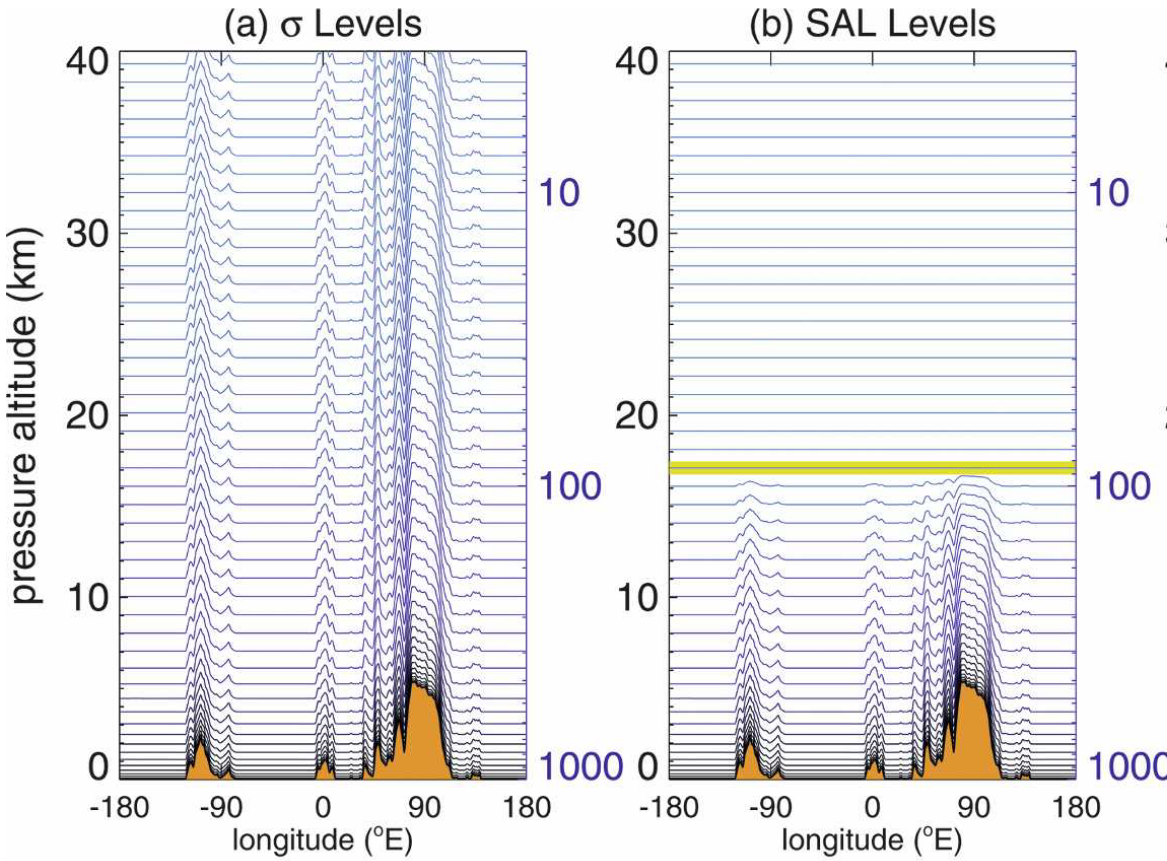
\includegraphics[width=0.55\textwidth]{figures/hybrid_sigma_pressure_layers.png}
  \end{center}
  \caption{Examples of (hybrid) sigma pressure layers. a) shows sigma layers like in Equation \ref{eq:sigma-definition}, while b) shows a hybrid approach in the form of Equation \ref{eq:hybrid-sigma} \cite{eckermann_hybrid_2009}}\label{fig:hybrid-sigma}
\end{figure}



This results in levels of equal pressure thickness, converging to isobaric layers at higher altitudes. 
Which exact form $A(\tilde{\eta})$ and $B(\tilde{\eta})$ took in the MPI GE CMIP6 could not be found in \cite{olonscheck_new_2023}, but every dataset using hybrid sigma pressure levels contains the variabels $ap(lev)$, $b(lev)$ and the field of pressure levels $ps(lon, lat, time)$, from which the pressure at any gridpoint and level can be calculated with 

\begin{equation}
\label{eq:mpige-sigma-hybrid-pressure}
p(lev, lon, lat, time) = ap(lev) + b(lev) ps(lon, lat, time)
\end{equation}


The top pressure can be ignored in this dataset since the upper border is zero.


\subsection{Structure of the data}


